\documentclass[12pt]{article}
\usepackage{fullpage}
\usepackage{graphicx}
\usepackage{hyperref}
\usepackage{bm}
\usepackage{amsmath}
\usepackage{amssymb}
\usepackage{derivative}
\usepackage{bm}
\usepackage{comment}
\usepackage{cancel}
\usepackage{xcolor}


\begin{document}
\title{General Relativity: Homework 1}
\author{Koichiro Takahashi}
\maketitle

\section*{Problem.1}
A curve in the x-y plane parameterized by $\lambda \in [-\frac{1}{2}, 1]$ is given by
\begin{gather*}
x(\lambda) = \lambda^2 - 1 \\
y(\lambda) = \frac{\lambda - 1}{\lambda + 1}
\end{gather*}
(1)
\begin{figure}[h]
  \begin{center}
  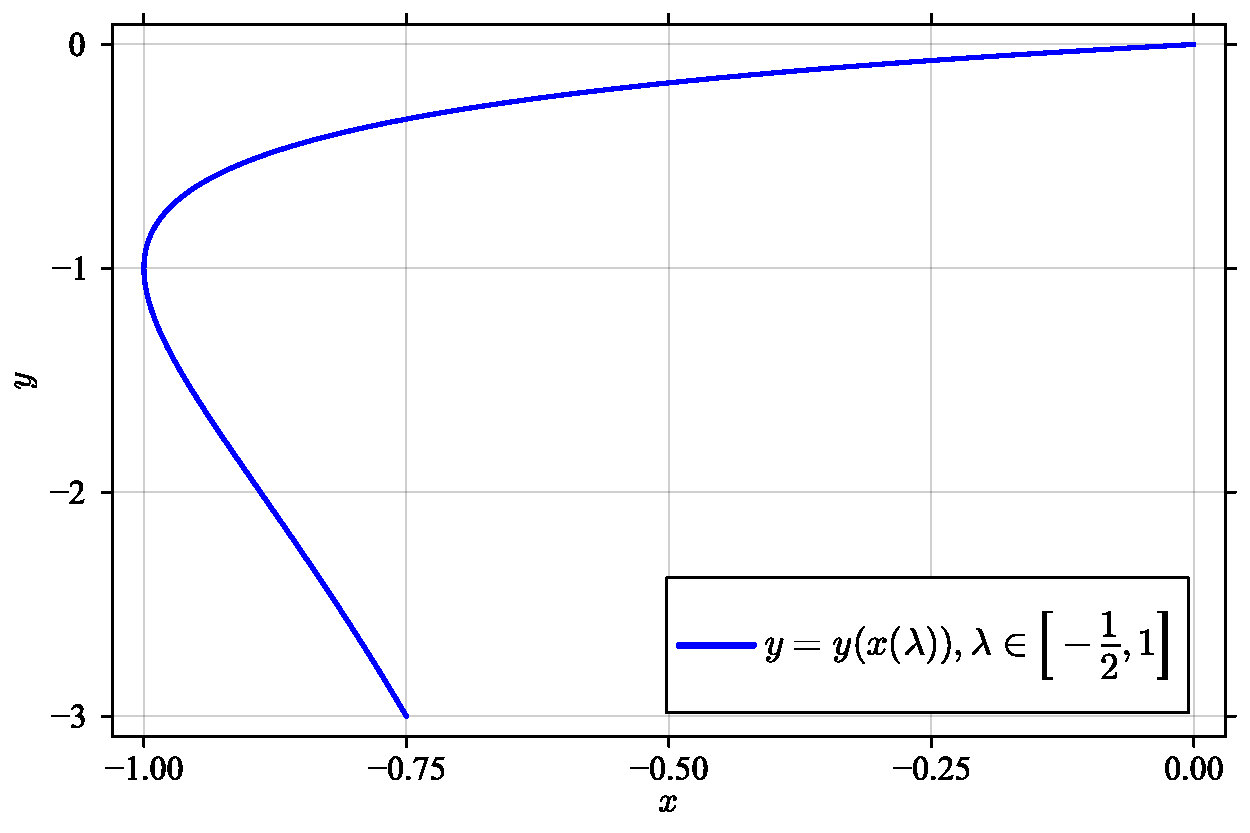
\includegraphics[width=0.7\linewidth]{Curves.pdf}
  \caption{Curves}
  \label{Curves}
  \end{center}
\end{figure}
\\
(2)
The tangent vector
\begin{gather*}
\Bar{T} = \left( \frac{d x}{d \lambda}, \frac{d y}{d \lambda}\right)
\end{gather*}
Here, 
\begin{gather*}
\frac{d x}{d \lambda} = \frac{d}{d \lambda} \left(\lambda^2 - 1 \right) = 2 \lambda \\[1em]
\frac{d y}{d \lambda} = \frac{d}{d \lambda} \left(\frac{\lambda - 1}{\lambda + 1} \right) = \frac{\left(\lambda + 1\right) - \left(\lambda - 1\right) }{\left(\lambda + 1\right)^2} = \frac{2}{\left(\lambda + 1\right)^2}
\end{gather*}
Therefore, the tangent vector at $\lambda = \frac{1}{2}$ is given by
\begin{gather*}
\Bar{T}\big|_{\lambda = \frac{1}{2}} = \left( \frac{d x}{d \lambda}, \frac{d y}{d \lambda}\right)\bigg|_{\lambda = \frac{1}{2}} = \left( 2 \lambda, \frac{2}{\left(\lambda + 1\right)^2}\right)\bigg|_{\lambda = \frac{1}{2}} = \left( 1, \frac{8}{9}\right)
\end{gather*}
(3)
The function $f$ is given by
\begin{align*}
f(x(\lambda),y(\lambda)) &= x(\lambda)^2 + 2x(\lambda)y(\lambda) - 3\\[1em]
&= \left(\lambda^2 - 1 \right)^2 + 2 \left(\lambda^2 - 1 \right) \left(\frac{\lambda - 1}{\lambda + 1} \right) - 3 \\[1em]
&=  \lambda^4 - 2 \lambda^2 + 1 + 2 \left(\lambda - 1 \right)^2 - 3\\[1em]
&=  \lambda^4 - 2 \lambda^2 + 1 + 2 \lambda^2 - 4 \lambda + 2  - 3 = \lambda^4 - 4 \lambda
\end{align*}
Therefore,
\begin{align*}
\frac{d f}{d \lambda} &= \frac{d}{d \lambda}  \left( \lambda^4 - 4 \lambda \right) = 4 \lambda^3 - 4 = 4\left(\lambda^3 - 1\right)
\end{align*}
At $\lambda = \frac{1}{2}$,
\begin{align*}
\frac{d f}{d \lambda}\bigg|_{\lambda = \frac{1}{2}} &= 4\left[\left(\frac{1}{2}\right)^3 - 1\right] = 4 \cdot \left(- \frac{7}{8} \right) = - \frac{7}{2}
\end{align*}
(4)
\begin{align*}
\frac{d f}{d \lambda} &= \frac{d}{d \lambda} f(x(\lambda),y(\lambda)) = \frac{\partial f}{\partial x} \frac{d x}{d \lambda} + \frac{\partial f}{\partial y} \frac{d y}{d \lambda} = \left( \frac{d x}{d \lambda}, \frac{d y}{d \lambda}\right) \cdot \left( \frac{\partial f}{\partial x}, \frac{\partial f}{\partial y}\right) = \Bar{T} \cdot \Bar{\nabla} f
\end{align*}

\section*{Problem.2}
The matrix $M$ and column vectors $U, V$ are given by
\begin{gather*}
M =
\begin{pmatrix}
3 & -1 & 0 & 0 \\
-1 & 1 & 0 & 0 \\
0 & 0 & 2 & 0 \\
0 & 0 & 0 & -1
\end{pmatrix}
, U =
\begin{pmatrix}
3\\ 2 \\ -2 \\ 0
\end{pmatrix}
, V =
\begin{pmatrix}
-1\\ 0 \\ 2 \\ 1
\end{pmatrix}
\end{gather*}
(1)
\begin{align*}
U^T V =
\begin{pmatrix}
3& 2 & -2 & 0
\end{pmatrix}
\begin{pmatrix}
-1\\ 0 \\ 2 \\ 1
\end{pmatrix}
= -3 + 0 - 4 + 0 = -7
\end{align*}
(2)
\begin{align*}
U V^T = 
\begin{pmatrix}
3\\ 2 \\ -2 \\ 0
\end{pmatrix}
\begin{pmatrix}
-1& 0 & 2 & 1
\end{pmatrix}
=
\begin{pmatrix}
-3 & 0 & 6 & 3 \\
-2 & 0 & 4 & 2 \\
2 & 0 & -4 & -2 \\
0 & 0 & 0 & 0
\end{pmatrix}
\end{align*}
(3)
\begin{align*}
U^T M V &= 
\begin{pmatrix}
3& 2 & -2 & 0
\end{pmatrix}
\begin{pmatrix}
3 & -1 & 0 & 0 \\
-1 & 1 & 0 & 0 \\
0 & 0 & 2 & 0 \\
0 & 0 & 0 & -1
\end{pmatrix}
\begin{pmatrix}
-1\\ 0 \\ 2 \\ 1
\end{pmatrix}
=
\begin{pmatrix}
3& 2 & -2 & 0
\end{pmatrix}
\begin{pmatrix}
-3 \\ 1 \\ 4 \\-1
\end{pmatrix}\\[1em]
&= - 9 + 2 - 8 + 0 = - 15
\end{align*}
(4)
The inverse matrix of $M$ is given by
\begin{align*}
M^{-1} = 
\begin{pmatrix}
1/2 & 1/2 & 0 & 0 \\
1/2 & 3/2 & 0 & 0 \\
0 & 0 & 1/2 & 0 \\
0 & 0 & 0 & -1 \\
\end{pmatrix}
\end{align*}
and it is unique. In fact, one can check that below:
\begin{align*}
\begin{pmatrix}
1/2 & 1/2 & 0 & 0 \\
1/2 & 3/2 & 0 & 0 \\
0 & 0 & 1/2 & 0 \\
0 & 0 & 0 & -1 \\
\end{pmatrix}
\begin{pmatrix}
3 & -1 & 0 & 0 \\
-1 & 1 & 0 & 0 \\
0 & 0 & 2 & 0 \\
0 & 0 & 0 & -1
\end{pmatrix}
=
\begin{pmatrix}
1 & 0 & 0 & 0 \\
0 & 1 & 0 & 0 \\
0 & 0 & 1 & 0 \\
0 & 0 & 0 & 1
\end{pmatrix}
= \mathbb{I}_{4\times4}
\end{align*}

\section*{Problem.3}
(1) In special relativity, laws of physics are the same in all inertial frames (any reference frame at constant velocity and constant angular velocity relative to a certain reference frame.)
\\
(2) The velocity Lorentz transformation into a frame which is moving at constant speed $v (\neq 0)$ relative to the original frame in the $x$ direction is given by
\begin{gather*}
\frac{d x'}{d t'} = \frac{\gamma \left(d x - v dt\right)}{\gamma \left(d t - v \frac{dx}{c^2}\right)} = \frac{\frac{d x}{d t} - v}{1 - \frac{v \frac{d x}{d t} }{c^2}}
\end{gather*}
By using the formula above, the velocity of $C$ as measured by $B$, denoted as $v_{CB}$ is obtained as below:
\begin{gather*}
v_{CB} = \frac{v_{CA} - v_{AB}}{1 - \frac{v_{AB} v_{CA} }{c^2}} = \frac{(-0.7c) - (0.8c)}{1 - \frac{(-0.7c) (0.8c) }{c^2}} = \frac{1.5c}{1 + 0.56} = -\frac{1.5c}{1.56} \approx -0.96 c 
\end{gather*}
Note that $v_{AB} = 0.8c, v_{CA} = -0.7c$.
\\
(3)
The electrostatic force 
\begin{gather*}
F = K \frac{q_1 q_2}{r^2}
\end{gather*}
is incompatible, since this physical quantity is NOT invariant under the Lorenz transformation, while special relativity requires that any physical quantity should not depend on the coordinate, i.e. invariant under the Lorentz transformation. (Any Lorentz-invariant quantity should be able to written down in tensor form...)
\\[1em]
In fact, one can perform the Lorentz transformation to the electrostatic force as follows.\\
If the distance $r$ between two point charges $q_1$ and $q_2$ in a reference frame is given by
\begin{gather*}
r = \sqrt{x^2 + y^2 + z^2}
\end{gather*}
where we define the four-dimensional coordinate $\Bar{x}$ as
\begin{gather*}
\Bar{x} = \left(t, x, y, z \right)
\end{gather*}
Then the Lorentz transformation into a frame which is moving at constant speed $v (\neq 0)$ relative to the original frame in the $x$ direction is given by
\begin{align*}
t' &= \gamma \left( t - \frac{v x}{c^2}\right)\\
x' &= \gamma \left( x - v t\right)\\
y' &= y\\
z' &= z\\
\gamma &= \frac{1}{\sqrt{1 - \frac{v^2}{c^2}}}
\end{align*}
and the inverse transformation is obtained by flipping the sign of $v$ and replacing the prime symbols, thus
\begin{align*}
t &= \gamma \left( t' + \frac{v x'}{c^2}\right)\\
x &= \gamma \left( x' + v t'\right)\\
y &= y'\\
z &= z'\\
\gamma &= \frac{1}{\sqrt{1 - \frac{v^2}{c^2}}}
\end{align*}
so that, $r$ in the new frame is
\begin{gather*}
r = \sqrt{\gamma^2 \left( x' + v t'\right)^2 + y'^2 + z'^2} \neq \left(t, x, y, z \right)
\end{gather*}
Therefore,
\begin{gather*}
F(t, x, y, z) \neq  F(t', x', y', z')
\end{gather*}
which means $F$ is NOT invariant under coordinate transformation.\\[1em]
(4)
The theory of electromagnetism is compatible with special relativity. The reason is the following. The Maxwell's equations are Lorentz invariant, i.e. the Maxwell's equations are invariant under Lorentz transformation, because you can write down the equations using the electromagnetic tensor $F^{\mu \nu}$. Thus the solution is also Lorentz invariant, which is consistent with special relativity.

\end{document}
